\documentclass[superscriptaddress,reprint,prb]{revtex4-1}
\usepackage{graphicx}
\usepackage[margin=0.7in]{geometry}
\usepackage{amsmath}
\usepackage{hyperref}
\usepackage{multirow}

\renewcommand{\Im}{\operatorname{Im}}
\renewcommand{\Re}{\operatorname{Re}}
\newcommand{\sub}[1]{\ensuremath{_{\textrm{#1}}}} %Upright multi-character subscript
\newcommand{\super}[1]{\ensuremath{^{\textrm{#1}}}} %Upright multi-character superscript

\newcommand{\HarvardSEAS}{John A. Paulson School of Engineering and Applied Sciences, Harvard University, Cambridge, MA, USA}
\newcommand{\MITPhy}{Department of Physics, Massachusetts Institute of Technology, Cambridge, MA, USA}

\usepackage[usenames]{color}
\newcommand{\TODO}[1]{\textcolor{red}{\textbf{TODO(#1)}}}
\newcommand{\edited}[1]{{\color{red} #1}}

\begin{document}

\title{Theory of phonon polaritons in polar dielectrics}

\author{Nicholas Rivera*}\email{nrivera@seas.harvard.edu}\affiliation{\HarvardSEAS}\affiliation{\MITPhy}
\author{Jennifer Coulter*}\email{jcoulter@g.harvard.edu}\affiliation{\HarvardSEAS}
\author{Prineha Narang}\email{prineha@seas.harvard.edu}\affiliation{\HarvardSEAS}


\date{\today}

\begin{abstract}
The ability to use photonic quasiparticles to control electromagnetic energy far below the diffraction limit is a defining paradigm in nanophotonics.  Largely, the manifestation of this idea has been plasmonics, which have been demonstrated to confine electromagnetic fields on the scale of nanometers. A more recent development is the measurement and manipulation of extremely confined phonon polariton modes in polar dielectrics such as silicon carbide and hexagonal boron nitride. These modes pave the way for nanophotonics and extreme light-matter interactions in the mid-IR to THz frequency band. To further advance this promising field, it is of great interest to compute the optical response of polar dielectrics from first principles. In this work, we develop linear response theory for an ionic lattice coupled to the electromagnetic field in arbitrary dimensions and derive expressions for the nonlocal dielectric function. While in some limits, our results qualitatively match the famous Lorentz oscillator model, we are able to specify its parameters in terms of the masses of the atoms in the unit cell, the tensor of Born effective charges of each atom in the unit cell,  phonon band-structure, and the phonon polarizations.  Moreover, our results allow us to point to a regime where quantum nonlocal effects may correct the phonon polariton dispersion, which may be relevant in experiments which confine electromagnetic fields to the scale of 1 nm. Our results also allow us for the first time to derive the dielectric function of phonon polaritons in a monolayer, which may also be specified in terms of ab-initio-derived parameters of the underlying lattice. We derive the electrodynamics of 2D phonon polaritons, finding their fields and dispersion. Finally, to show the practical usage of the framework derived, we provide ab-initio calculations for silicon carbide, and show that they agree well with experimental data.
\end{abstract}

\maketitle

Phonon polaritons, hybrid quasiparticles of photons and optical phonons, offer great promise for deeply sub-diffractional control of electromagnetic fields at mid-IR and THz frequencies. These polaritons share many features in common with plasmon-polaritons in conductors, a heavily well-studied topic. Namely, in recent years, it has been shown that phonon polaritons offer the ability to confine light to volumes over $10^6$ times smaller than that of a photon in free-space at the diffraction limit \cite{caldwell2013low,xu2014mid,caldwell2014sub,dai2014tunable,tomadin2015accessing,yoxall2015direct,li2015hyperbolic,dai2015subdiffractional,dai2015graphene,caldwell2015low,li2016reversible,Basov:2016,basov2017towards,low2017polaritons,giles2017ultra}. Because of this, and their relatively high lifetimes of around picoseconds, they allow new opportunities for vibrational spectroscopy, for radiative heat transfer \cite{hillenbrand2002phonon}, and for control of dynamics in quantum emitters \cite{kumar2015tunable,rivera2017making}. Largely, the core features of phonon polaritons, such as mode shape, confinement, and propagation characteristics, can be understood through the properties of the Lorentz oscillator dielectric function, which has been successfully applied to model experiments involving the launching and propagation of these polaritons.

There are nevertheless some outstanding questions regarding the behavior of phonon polaritons. Here, we present a few. 
\begin{enumerate}
\item{Can the very successful Lorentz oscillator model ever break down? One particular mechanism of breakdown, which could be present in the case of extremely confined polaritons, concerns effects coming from spatial dispersion. Such short phonon polariton wavelengths are indeed predicted by classical electrodynamics of a polar dielectric, especially in the case of a very thin film (nm-thick).}
\item{What are the properties of phonon polaritons in reduced dimensions, such as 2D polar insulators? Can they support extremely confined polaritonic modes, in analogy to extremely confined plasmonic modes in 2D plasmonic materials such as graphene?}
\item{In general, are the properties of optical phonons inherited by the phonon polariton? What is the influence of concepts such as interface phonons and phonon topology on the polariton? The ability to design new phonon polariton materials by designing the optical phonon band structure allows a predictive way to generate polaritonic materials.}
\end{enumerate}

Indeed, the way to proceed on all of these questions is an ab-initio framework to predict the phonon contribution to the dielectric tensor in arbitrary settings. Frameworks exist for calculating the local permittivity coming from phonons in a 3D bulk, as in \cite{Gonze1997dynamical}, and implemented in software packages such as ABINIT \cite{abinit1,abinit2,abinit3}. Here, we develop a unified 
theoretical framework to analyze phonon-polaritons in materials, which can address effects of spatial dispersion as well as effects coming from arbitrary dimensionality. Specifically, we develop a means to arrive at the dielectric function associated with optical phonons in two- and three-dimensional materials. We pay close attention to develop a description of the optical response that shows clearly the parallels to the description of plasmonic response from first principles. From this theory, we not only accurately predict surface phonon polaritons in thick materials where a bulk permittivity is valid  but also provide tools to predict phonon polariton dispersion in monolayers and anticipate when spatially nonlocal corrections to the phonon contribution to the dielectric function become relevant. 

\section{Linear response of phonon polaritons in three dimensions}

\textcolor{blue}{Pri: one place we can get criticized here by an experimentalist (or theorist) is that at least for the 3D spatially-local case, there's this thing that Caldwell called the TO-LO formalism in his proposal. It's not actually a formalism... it's just an expression for the dielectric function in terms of the high-frequency electronic part, and the various TO and LO phonon frequencies, as well as the damping. It features some fairly simple-to-get experimental parameters (though actually I don't know how they get the LO frequency since only TO comes up in Raman I think), and reproduces the data generally pretty well. I think actually this is what they did in that arXiv paper that worried us about a month ago. Anyway, when we do nonlocal and reduced-dimensional stuff, I think this is where we can really be different. In any event, it's good to anticipate this criticism in advance so we can potentially get in front of it. What do you think?}

\textcolor{blue}{To all: I'm new to phonons and am likely making some non-standard notational choices? If so, feel free to point out where and I'll try to standardize it.} We start by reviewing the theory of phonon polaritons in a 3D bulk, developing the theory in a way that is parallel to the linear response theory of electronic contributions to the permittivity and plasmonic properties. Here, the matter subsystem which couples to light is the ionic lattice of the crystal. Thus, we develop the linear response theory of an ionic lattice to an electromagnetic field. The interaction Hamiltonian of the lattice with the electromagnetic field is taken as
\begin{equation}
H_{int} = -\int d^3x ~\mathbf{E}(\mathbf{x},t)\cdot\mathbf{P}(\mathbf{x},t),
\end{equation}
where $\mathbf{E}$ is a driving electric field, and $\mathbf{P}$ is the polarization associated with the lattice. We write the polarization as a sum of contributions from all unit cells in the system. Namely
\begin{equation}
\mathbf{P}(\mathbf{r},t) = \sum\limits_{\text{sites, }\mathbf{R}}\mathbf{d}(\mathbf{R},t)\delta(\mathbf{r}-\mathbf{R}),
\end{equation}
where $\mathbf{d}(\mathbf{R},t)$ is the time-dependent dipole moment associated with lattice site $\mathbf{R}$. In expressing the polarization in this fashion, we are assuming that the displacement of the ions is far smaller than the size of the unit cell, which is, even in a deeply anharmonic regime, a good approximation. This said, we operate in the harmonic regime.  The dipole moment is given by $\mathbf{d}(\mathbf{R},t) = \sum\limits_{\text{basis sites,}\kappa} \mathbf{b}_{\kappa} \mathbf{Z}_{\kappa}\mathbf{u}(\mathbf{R}_{\kappa} \equiv \mathbf{R}+\mathbf{b}_{\kappa},t)$, where $\mathbf{Z}_{\kappa}$ is the tensor of Born effective charges for atom $\kappa$ in the unit cell at basis vector $\mathbf{b}_{\kappa}$ and $\mathbf{u}(\mathbf{R}_{\kappa},t)$ is the displacement of atom $\kappa$ at basis site $\mathbf{R}_{\kappa}$. Note that the Born effective charges are both tensorial and site-dependent. \textcolor{blue}{I still want to give a decent intuition for these Born effective charges as I find them a bit mysterious and so will a reader who is from photonics.} This displacement can be expanded in phonon modes as
\begin{equation}
\mathbf{u}(\mathbf{R}_{\kappa},t) = \sum\limits_{\mathbf{q}\sigma}\sqrt{\frac{\hbar}{2M_{\kappa}N\omega_{\mathbf{q}\sigma}}}\left( e^{i\mathbf{q}\cdot\mathbf{R}_{\kappa}-i\omega_{\mathbf{q}\sigma}t}\hat{e}_{\mathbf{q}\sigma}(\mathbf{b}_{\kappa})a_{\mathbf{q}\sigma} + \text{h.c.} \right),
\end{equation}
where $M_{\kappa}$ is the mass of atom $\kappa$, $\omega_{qs}$ is the phonon frequency at wavevector $\mathbf{q}$ and branch $s$, and $N$ is the number of unit cells.
Assuming that the field is weak, the expectation value of the polarization in the lattice will depend linearly on the total field acting on the ions: this field is the sum of the external field with the field resulting from induced electronic and ionic polarization, and it is this field which appears in the interaction Hamiltonian of Equation (1). We define the linear-response relation for a bulk crystal in Fourier space as $\langle\mathbf{P}(\mathbf{q},\omega)\rangle = \epsilon_0\boldsymbol{\Pi}(\mathbf{q},\omega)\mathbf{E}(\mathbf{q},\omega)$, where we refer to $\boldsymbol{\Pi}(\mathbf{q},\omega)$ as the polarization-polarization response function.

To connect this polarization-polarization response function to the observed dielectric function, we write down Maxwell's equations for the electric field sourced by a polarization density. We have that
\begin{equation}
\left(-\mathbf{q}\times\mathbf{q}\times - \epsilon_{\infty}\frac{\omega^2}{c^2} \right)\mathbf{E} = \omega^2\mu_0\mathbf{P}(\mathbf{q},\omega),
\end{equation}
where $\omega$ is the frequency of light under consideration $\mathbf{P}$ is the polarization at that frequency, and $\epsilon_{\infty}$ is the high-frequency dielectric function associated with the electrons. Now, we identify the average polarization $\langle\mathbf{P}\rangle$ with the classical polarization $\mathbf{P}$ in Maxwell's equations. We note that an analogous procedure is also employed in the linear-response theory of the longitudinal response of electrons, where instead of the polarization density being averaged, the charge density is averaged. And instead of the solving Maxwell's equations for the field, one solves Laplace's equation for the potential.  Using the linear response relation $\mathbf{P} = \epsilon_0\boldsymbol{\Pi}\mathbf{E}$, we have simply that
\begin{equation}
\left(-\mathbf{q}\times\mathbf{q}\times - \left(\epsilon_{\infty} + \boldsymbol{\Pi} \right)\frac{\omega^2}{c^2}\right)\mathbf{E} = 0,
\end{equation}
leading to the identification of of the dielectric tensor $\boldsymbol{\epsilon} = \epsilon_{\infty} + \boldsymbol{\Pi}$. 

Now, we determine the polarization-polarization response function. It is given by the Kubo formula at finite temperature via
\begin{equation}
\boldsymbol{\Pi}(\mathbf{q},\omega) =  \frac{1}{\epsilon_0 V}\sum\limits_{m,n}\frac{\mathbf{P}_{mn}(\mathbf{q})\otimes\mathbf{P}_{nm}(\mathbf{q})}{\hbar\omega + E_{nm}+i\frac{\Gamma}{2}}\left(e^{\beta E_m}-e^{\beta E_n} \right),
\end{equation}
%where $\Gamma$ is a positive infinitesimal, and it is to be understood that rigorously, the limit $\Gamma \rightarrow 0$ is to be taken. In a situation where there is phonon dissipation, typically due to electron-phonon and phonon-phonon scattering, we make take a relaxation-time approximation and interpret $\Gamma$ as the finite relaxation time. 
where $m$ and $n$ are taken to be eigenstates of the lattice, $V$ is a normalization volume, and we have written the polarization-polarization susceptibility in Fourier space. It is  understood that the polarization operator is now the Schrodinger operator. $\Gamma$ is a positive infinitesimal, and it is to be understood that rigorously, the limit $\Gamma \rightarrow 0$ is to be taken. In a situation where there is phonon dissipation, typically due to electron-phonon and phonon-phonon scattering, we make take a relaxation-time approximation and interpret $\Gamma$ as the finite relaxation time.   The eigenstates span the phononic Fock space. For simplicity, we will work at zero temperature from here onwards. In this case, in the first term, the states $m$ must be zero-phonon states, while in the second term, the states $n$ must be zero-phonon states. Due to the displacement being linear in creation and annihilation operators, the states $n$ and $m$ in the first and second terms (resp.) must be one-phonon states. The Fourier transformed polarization operators are found to be
\begin{equation}
\mathbf{P}(\mathbf{q}) = \sum\limits_{\mathbf{R}}\mathbf{d}(\mathbf{R})e^{-i\mathbf{q}\cdot\mathbf{R}} \equiv \mathbf{d}(\mathbf{q}),
\end{equation}
where it is to be understood that $\mathbf{P}(\mathbf{q})$ refers to a continuous Fourier transform while $\mathbf{d}(\mathbf{q})$ refers to a discrete Fourier transform. Plugging in the displacement operator of Equation (3), one finds that $\mathbf{d}(\mathbf{q})$ is given by
\begin{equation}
\mathbf{d}(\mathbf{q}) = \sum\limits_{\sigma}\sqrt{\frac{\hbar N}{2\omega_{\mathbf{q}\sigma}}} \left(\mathbf{S}_{\mathbf{q}\sigma}a_{\mathbf{q}\sigma} + \text{h.c.}\right),
\end{equation}
where 
\begin{equation}
\mathbf{S}_{\mathbf{q}\sigma} = \sum\limits_{\kappa} \frac{1}{\sqrt{M_{\kappa}}}\mathbf{Z}_{\kappa}\hat{e}_{\mathbf{q}\sigma}(\mathbf{R}_{\kappa}).
\end{equation}
This can be expressed in terms of more standard outputs of ab-initio software that calculates phonon properties. In particular, we can take $\hat{e}_{\mathbf{q}\sigma}$, the eigenvectors of the dynamical matrix, and define eigendisplacements via $\boldsymbol{\eta}_{\mathbf{q}\sigma\kappa}=\frac{\hat{e}_{\mathbf{q}\sigma}}{\sqrt{M_{\kappa}}}$. In which case, we may cast Equation (9) into the form:
\begin{equation}
\mathbf{S}_{\mathbf{q}\sigma} = \sum\limits_{\kappa} \mathbf{Z}_{\kappa}\boldsymbol{\eta}_{\mathbf{q}\sigma\kappa}.
\end{equation}
We may now use this in concurrence with Equation (6) to evaluate the dielectric function. Consider $\boldsymbol{\Pi}(\mathbf{q},\omega)$. From the form of Equation (8), we see that at zero temperature, the first term only sees contributions from $m=|0_{\mathbf{q}\sigma}\rangle$ and $n=|1_{\mathbf{q}\sigma}\rangle$, where $0_{\mathbf{q}\sigma}$ and $1_{\mathbf{q}\sigma}$ refer to the number of phonons in mode $\mathbf{q}\sigma$. Here $\sigma$ can be any branch of the phonon band structure. In the second term, $m$ and $n$ switch. In the limit where the phonons are very weakly damped, $\Gamma_{\mathbf{q}\sigma} \\ \omega_{\mathbf{q}\sigma}$. this leads to:
\begin{equation}
\boldsymbol{\Pi}(\mathbf{q},\omega) = \frac{1}{\Omega}\sum\limits_{\sigma}\frac{\mathbf{S}_{\mathbf{q}\sigma}\otimes \mathbf{S}_{\mathbf{q}\sigma}^*}{\omega^2_{\mathbf{q}\sigma}-\omega^2-i\Gamma_{\mathbf{q}\sigma}\omega},
\end{equation}
where $\Omega=N/V$ is the volume of the unit cell. Rigorously, the phonon frequencies in this equations are real. However, in the realistic situation where there is phonon dissipation, typically due to electron-phonon and phonon-phonon scattering, we may make take a "relaxation-time approximation" which effectively results in expressing $\omega_{\mathbf{q}\sigma} \rightarrow \omega_{\mathbf{q}\sigma} - i\frac{\Gamma_{\mathbf{q}\sigma}}{2}$, where $\Gamma_{\mathbf{q}\sigma}$ is the dissipation rate of the phonon. Finally, the dielectric function takes the form
\begin{equation}
\epsilon(\mathbf{q},\omega) = \epsilon_{\infty} + \frac{1}{\Omega}\sum\limits_{\sigma}\frac{\mathbf{S}_{\mathbf{q}\sigma}\otimes \mathbf{S}_{\mathbf{q}\sigma}^*}{\omega^2_{\mathbf{q}\sigma}-\omega^2-i\Gamma_{\mathbf{q}\sigma}\omega}.
\end{equation}
From this equation, let us consider an extremely simplified limit. Assume that the permittivity is isotropic. Further assume that the site-specific masses collapse to a single effective mass $M^*$, and that the site-specific and tensorial Born effective charges collapse to a single effective charge $Q^*$. Finally, assume that the only phonon with oscillator strength (non-zero $\mathbf{S}$) is the transverse optical phonon at frequency $\omega_{TO}$. In this case, one arises at a dielectric function 
\begin{equation}
\epsilon(\omega) = \epsilon_{\infty} + \frac{NQ^{*2}}{\epsilon_0 M^*V}\frac{1}{\omega^2_{TO}-\omega^2-i\Gamma_{TO}\omega},
\end{equation}
which coincides precisely with the phenomenological Lorentz oscillator model, showing the consistency, of our approach. That said, our approach takes into account complications arising from the tensorial and site-dependent nature of the Born charges, the effects of a complex unit-cell, as well as a detailed understanding of the phonon band-structure and how it affects the features of the predicted dielectric function.

Before applying this formalism to a real material and also before discussion of the two-dimensional case, we briefly comment on "nonlocality" in the phonon contribution to the dielectric function. 
\textcolor{blue}{Should this part below be moved to the outlook or does it make sense to be here instead?} Note that Equation (12) has a wavevector dependence which is implicit through the phonon dispersion. As a result, the phonon contribution to the dielectric function sees contributions from the entire phonon band structure, including the large wavevector components. However, $\epsilon(\mathbf{q},\omega)$ measures the response to an electromagnetic perturbation of frequency $\omega$ and wavevector $\mathbf{q}$. In the vast majority of experiments that have been performed on phonon polaritons, the wavevector used to probe the polariton is on the order of $\frac{\omega}{c}$ which is much less than the wavevector scale at which the optical phonon dispersion varies, which is of the order of $\frac{\pi}{a}$ where $a$ is a lattice constant of the polar dielectric.  Even in scattering near-field optical microscope experiments, where one uses an AFM tip of radius of about $20$ nm to probe the polaritons, the wavevectors accessed would still be extremely small compared to the extent of the Brillouin zone. It would then seem almost hopeless to see nonlocal behavior for the phonon-polaritons. However, a recent experiment \cite{iranzo2018probing} has shown that plasmons in graphene, by means of a gold mirror, can be confined to dimensions of about 1 nm in the dimension transverse to the graphene sheet. Additionally, another recent experiment \cite{benz2016single} has leveraged so-called "picocavities", sub-nanometer gaps between a metal nanoparticle and metal film, to access very strong light-matter couplings and extreme variations in fields. These two experiments show a way to get large optically-accessed wavevectors to probe nonlocal behavior in polar dielectrics.

\section{Application to silicon carbide}
% calculation basics
To demonstrate the practical use of this theoretical framework, we present an example bulk calculation for the 4H polytype of silicon carbide (SiC), whose unit cell is shown in Figure 1(a).  %Calculations of the frequency-dependent dielectric tensor 
Phonon bandstructure of SiC were performed within density functional perturbation
theory (DFPT) as implemented in the ABINIT package\cite{abinit1,abinit2,abinit3,Gonze1997dynamical,Hamann2005metric}, with electric field response included to appropriately capture LO-TO splitting. Initial ground state density functional theory (DFT) properties were predicted using the PBEsol parameterization of the norm-conserving Vanderbilt pseudopotentials \cite{PBEsol,ONCV_PPs,pseudodojo}. We calculated the phonon modes, their frequencies (shown in Figure 1(b)), and their eigendisplacements at the gamma point to construct the dielectric function from Equation (12), using experimental values for the dissipation rates $\Gamma$. We note that while here, we have taken both the SiC bandgap and the SiC optical phonon lifetime from experiments, these quantities may also be obtained ab-initio by calculating lifetimes associated with electron-phonon scattering and three-phonon decay processes. 

\begin{figure}[t]
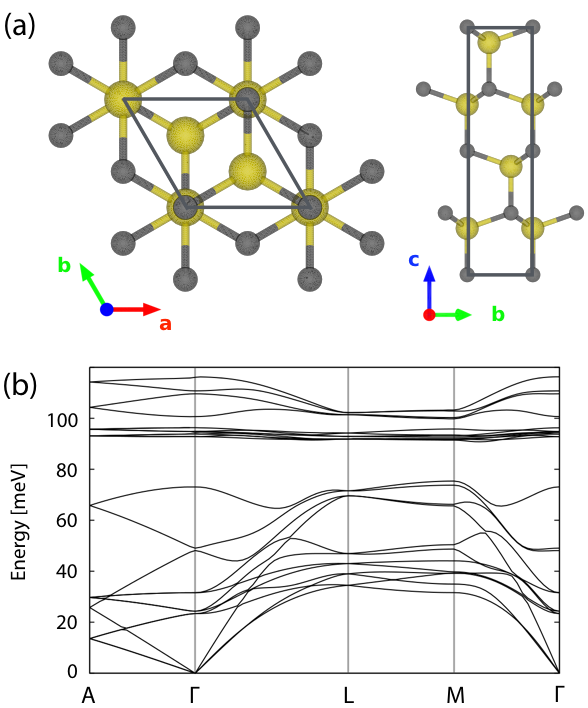
\includegraphics[width=8cm]{structure.png}
\caption{\textbf{Crystal structure and phonon dispersion of 4H silicon carbide.} a) The hexagonal unit cell structure of silicon carbide allows different optical response in the a-b plane and along the c axis. b) The full phonon bandstructure of silicon carbide, from which the phonon eigendisplacements associated with the gamma point were used to calculate the frequency-dependent dielectric function.}
\label{fig:phonons}
\end{figure}

% about the scissor shift -- and a defense sentence in case someone hits us with "semi-empirical" later on
Additionally, a scissor shift of 1.01 eV was applied to shift the calculated band gap of 2.26 eV to match the experimental gap of $\sim$3.27 eV \cite{band_gap_expt1,band_gap_expt2}. This is necessary to correct for the well-known underestimation of the band gap in ground state density functional theory calculations and the corresponding effects to the dielectric response.
The high-frequency dielectric tensor was found to be $\epsilon^{\infty}_{\parallel}$ = 6.986 and $\epsilon^{\infty}_{\perp}$ = 7.307.  This also leads to a modification of the phonon spectra. % For a material in which the band gap is not as well known as in SiC, a more computationally intensive GW calculation could be used for an entirely \it{ab initio} implementation of our theory. If excitonic effects contribute significantly to the optical properties of a chosen material, a Bethe-Salpeter prediction might be used to further improve predictive accuracy. 
The resulting frequency-dependent dielectric tensor, compared to experimental values from \cite{tiwald1999carrier}, is shown in Figure \ref{fig:epsilon}. As can be seen, the agreement between the theoretical calculation and the experimental results is quite good. 




\textcolor{red}{ Should we mention here that while we take the dissipation rate and bandgap from experiment, that these quantities can be obtained ab initio as well? We could cite packages that would allow someone to do this for a material where properties aren't well known, just to keep ourselves in the "first principles" designation. Maybe a note in the supplement or a footnote with this to prevent "semi-empirical" finger pointing?}

\textcolor{blue}{I included a sentence addressing this important point after the sentence where we say that we take the lifetimes from experiment. }

% can also put this table just by listing eps^inf_perp and parallel in the main text.  
\begin{figure}[t]
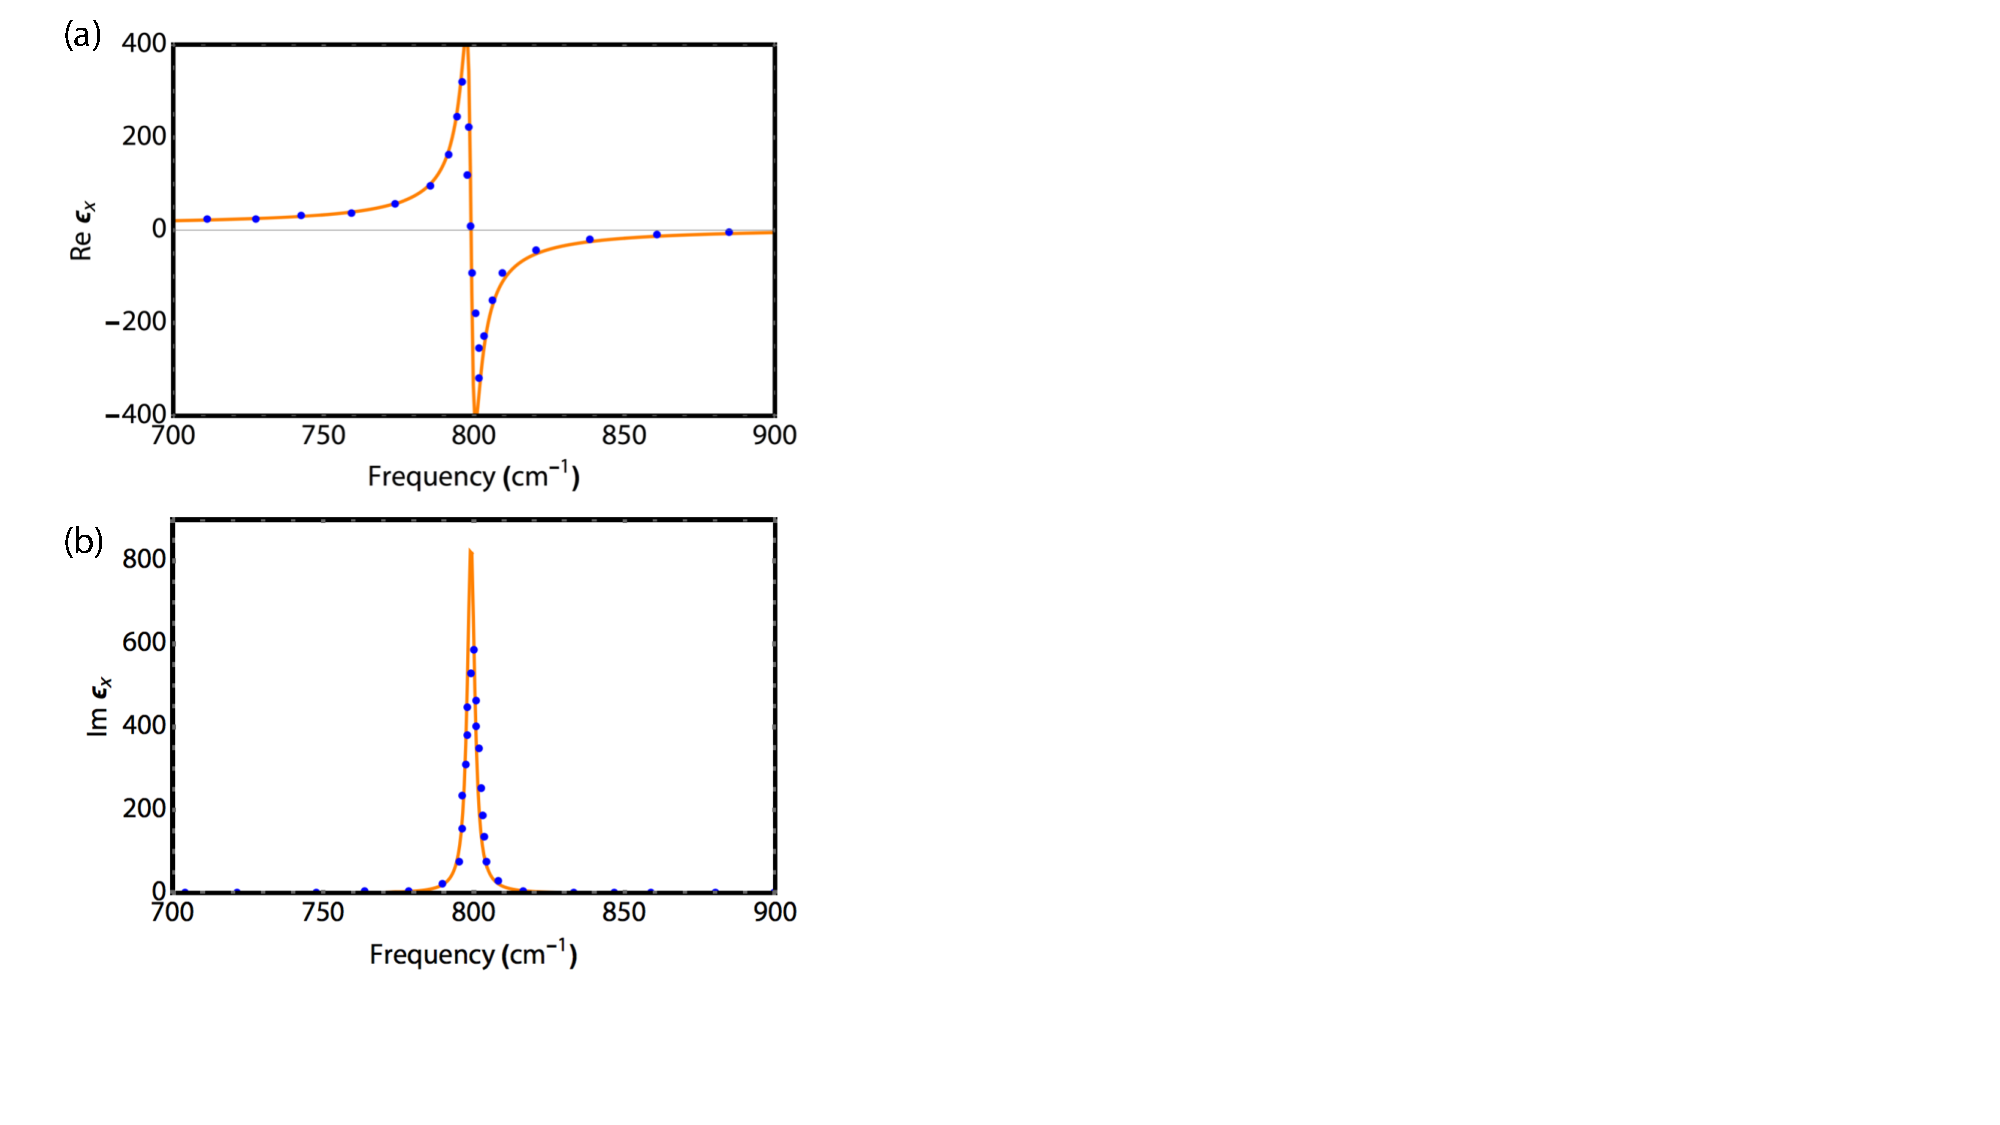
\includegraphics[width=8.5cm]{SiC_comparison_thy_vs_expt.pdf}
\caption{\textbf{Comparison of theoretical predictions and experimental values of the infrared dielectric function of bulk 4H silicon carbide.} The frequency-depended dielectric tensor in the direction perpendicular to the c-axis (orange), calculated for bulk 4H silicon carbide from using Equation (12). The phonon properties and $\epsilon_{\infty}$ calculated from the ABINIT package. Overlaid in blue dots are the experimental values for the dielectric function, taken from \cite{tiwald1999carrier}. The real part is shown in (a) while the imaginary part is shown in (b). }
\label{fig:epsilon}
\end{figure}

%Thus, to evaluate it, we must know the microscopic states of the lattice, in addition to matrix elements of displacement. Working in the harmonic approximation, the states are simply phonon-occupation states $|\{n_{qs}\}\rangle$, labeled by their wavevector $\mathbf{q}$ in the Brillouin zone and their band $s$ which encodes transverse/longitudinal polarization of acoustic/optical branches. The phonons are also labeled by their frequency $\omega_{qs}$ and the polarization vector at each basis site $b$, $\hat{e}_{\mathbf{q}s}(\mathbf{b})$. The displacement of each ion in the lattice can be expressed as an expansion over phonon modes as:
% \begin{equation}
% \mathbf{u}(\mathbf{R},\mathbf{b},t) = .
% \end{equation}
% From the displacement, we then must construct the dipole moment associated with each unit cell in the lattice. This is given by:
% \begin{equation}
% \mathbf{d}(\mathbf{R}) = e\sum\limits_{\mathbf{b}} Z_{ij}u_{j},
% \end{equation}
% where $\mathbf{Z}$ is a tensor of Born effective charges. These charges formally are defined as the derivative of the lattice polarization with respect to charge displacement. They act as effective charges for the ions, taking into account the motion of electrons and other ions in the system. Once we have the dipole moment in each unit cell, we can now complete the formal evaluation of the polarization-polarization response function. Assuming that we are operating at zero temperature, it is given by:

\section{Linear response of phonon polaritons in two dimensions}
We now move to generalize the derivation of the previous section to describe the optical phonon contribution to Maxwell's equations coming from a two-dimensional material. Because of the change of symmetry in the system, we will not be able to perform the analysis by Fourier transforming Maxwell's equations in three dimensions. However, we will apply a technique which is often used to analyze electromagnetic modes in 2D systems such as plasmons in 2D conductors. An example of the technique is shown in detail in \cite{jablan2009plasmonics}, but we summarize the essential details here. 

Consider a two-dimensional ionic lattice located in the $xy$ plane ($z=0$) surrounded by a homogeneous environment of permittivity $\epsilon$. We consider the simplified case where the lattice is free-standing, to show the essential concept. We search for a mode whose magnetic field $\mathbf{H}$ is of the form $\mathbf{H}(z)e^{i\mathbf{q}\cdot\mathbf{r}_{||}-i\omega  t}$, where $\mathbf{r}_{||}=(x,y,0)$ is the position in the plane, $\mathbf{q}$ is the wavevector and $\omega_{\mathbf{q}}$ is the frequency. To simplify the discussion even further and furnish analytical forms for the phonon-polariton modes in 2D, we assume this material has mirror symmetry along the axis of $\mathbf{q}$. In this case, the electromagnetic modes can be decomposed into TE and TM-polarized modes. As is typical in the study of highly-confined polaritons, whether they are plasmon- or phonon- polaritons, the TM mode is the highly confined one, and occurs when $\epsilon < 0$. In our convention, the TM mode is such that $\mathbf{H}$ is in the plane of the lattice and perpendicular to $\mathbf{q}$. Without loss of generality, define the $\mathbf{q}$ direction to be the $x$ direction, making the magnetic field in the $y$ direction. Moreover, the magnetic field in this mode flips sign under $z \rightarrow -z$. 

For $z \neq 0$, the Maxwell equation for the magnetic field is $(\nabla\times\nabla\times - \epsilon\frac{\omega^2}{c^2})\mathbf{H} = 0$. This equation, for the TM mode described above, becomes 
\begin{equation}
\left(-\frac{d^2}{dz^2}+\mathbf{q}^2-\epsilon\frac{\omega^2}{c^2} \right)H = 0,
\end{equation}
where we have written $\mathbf{H} = H\hat{y}$. The solution in the region $z > 0$ is simply \begin{align}
H &= e^{i\mathbf{q}\cdot\mathbf{r}_{||}-\kappa z}, ~z>0 \nonumber \\
H &= -e^{i\mathbf{q}\cdot\mathbf{r}_{||}-\kappa z}, ~z>0 \nonumber \\
\end{align}
where $\kappa = \sqrt{\mathbf{q}^2-\epsilon\frac{\omega^2}{c^2}}$ and we have implicitly assumed $q > \epsilon\frac{\omega}{c}$ as we are interested in confined evanescent modes. To join these two solutions consistently, we apply the interface conditions for the magnetic field. They are $\hat{z}\times(\mathbf{H}^{(+)}-\mathbf{H}^{(-)}) = \mathbf{K} = -i\omega\mathbf{P}_s$ where $\mathbf{K}$ is the surface current density, expressed through the surface polarization density $\mathbf{P}_s$. 
Now we use the linear response relation $\mathbf{P}(\mathbf{q},\omega) = \boldsymbol{\Pi}(\mathbf{q},\omega)\mathbf{E}(\mathbf{q},\omega)$ in addition to Ampere's law $\nabla\times\mathbf{H} = -i\omega\epsilon\mathbf{E}$. Plugging these relations in yields an implicit equation connecting the polarization response function, the frequency of the 2D phonon polariton, and its frequency. Taking the case where $x$ coincides with a principal axis of the system, we have that 
\begin{equation}
q\Pi_{xx}(q,\omega)  = -2\epsilon.
\end{equation}

To connect this relation to the discussion of the three-dimensional case, we write a microscopic form for the polarization response function of the ionic lattice. It is simply
\begin{equation}
\boldsymbol{\Pi}(\mathbf{q},\omega) =  \frac{1}{\epsilon_0 A}\sum\limits_{m,n}\frac{\mathbf{P}_{mn}(\mathbf{q})\otimes\mathbf{P}_{nm}(\mathbf{q})}{\hbar\omega + E_{nm}+i0^+}\left(e^{\beta E_m}-e^{\beta E_n} \right),
\end{equation}
where the only change is to replace a normalization volume with a normalization area $A$. Here, $\mathbf{P}(\mathbf{q})$ is the 2D Fourier transform of the polarization density. As the form of the displacement of the ions is still given by Equation (3), $\mathbf{P}(\mathbf{q})$ is still given by Equations (7-10), but with the Born charges and eigendisplacements appropriate to the 2D system of interest. Note that although the lattice is two dimensional, in general, the ions may be displaced in any three directions and thus $\boldsymbol{\Pi}$ is still a $3\times3$ matrix. Following the same kind of reasoning that lead to Equation (13), if we parameterize the effect of the different masses and Born charges in the unit cell by $M^*$ and $Q^*$, we will find a form for the polarization response function which is given by the second term of Equation (13) but with $V$ replaced by $A$. Defining $N/A \equiv n_s$, Equation (14) for the dispersion relation of 2D phonon polaritons tells us that
\begin{equation}
\omega = \sqrt{\omega_{TO}^2+\frac{n_sQ^{*2}}{2M^*\epsilon_0\epsilon}q}.
\end{equation}
Note that this dispersion has a strong resemblance to the plasmon dispersion relation of two-dimensional electron gases, which is normally of the form $\omega = \sqrt{\frac{n_s e^2  }{2m\epsilon_0\epsilon}q}$ \cite{stern1967polarizability}. The only difference is the replacement of electron parameters (density, charge, mass) by the corresponding lattice parameters in the phononic case, and a shift in the minimum frequency by the transverse optical phonon frequency.

\textcolor{blue}{Still looking for more to say about this. This probably requires some brainstorming discussion between us. For now, what I'll do is prepare a plot of the Fourier transform of the green's function of the Maxwell equations for the 2D sheet (p-polarized reflectivity, as was done in Argentene).} 

% We now move to generalize the derivation of the previous section to describe the optical phonon contribution to Maxwell's equations coming from a two-dimensional material. Because of the change of symmetry in the system, we will not be able to perform the analysis by Fourier transforming Maxwell's equations in three dimensions. Nevertheless, we may proceed as follows. Consider Maxwell's equations with a source density given by
% \begin{equation}
% \mathbf{P}(\mathbf{r}) = \mathbf{P}(\mathbf{r}_{||})\delta(z) = \sum\limits_{\mathbf{R}}\mathbf{d}(\mathbf{R})\delta(\mathbf{R}-\mathbf{r})\delta(z).
% \end{equation}
% Taking the fourier transform in two dimensions gives:
% \begin{equation}
% \mathbf{P}(\mathbf{q},\omega) = \delta(z)\sum\limits_{\mathbf{R}}\mathbf{d}(\mathbf{R})e^{-i\mathbf{q}\cdot\mathbf{R}}.
% \end{equation}
% Fourier transforming the Maxwell equations in two dimensions, leaving the third unchanged connects the fourier transformed polarization density to the  
% \begin{equation}
% \left(-\frac{d^2}{dz^2} + \mathbf{q}^2 - \frac{\omega^2}{c^2} \right)\mathbf{E}(\mathbf{q},\omega) = \mu_0\omega^2\mathbf{P}(\mathbf{q},\omega)\delta(z)
% \end{equation}
% To connect to response functions, we note that: the Hamiltonian is given by Equation (1), integrated over two dimensions, the linear response relation is $\langle \mathbf{P}(\mathbf{q},\omega) = \epsilon_0\boldsymbol{\Pi}(\mathbf{q},\omega)\mathbf{E}(\mathbf{q},\omega)$, and that the susceptibility is still defined by Equation (6), except that the units of the polarization density are different, and the volume factor becomes an area factor $A$. Given this 2D polarizability of the ionic lattice, we may solve Maxwell's equations for the resultant fields, as well as the dispersion relation of the phonon-polariton modes. We consider for simplicity an isotropic case

%While we could work in Fourier space in two dimensions and real-space in the third, we employ a simpler argument for the phonon-polariton modes of a 2D structure and the response function that captures such phonon-polariton response.

%In particular, what we will do is, in the spirit of the self-consistent mean-field approximation, find an expression for the expectation value of the dipole moment at each site in the two-dimensional lattice. Then, using Maxwell's equations, write the electromagnetic field as a superposition of fields from the various dipoles. In particular, suppose we have a two-dimensional lattice with sites $\mathbf{R}$ in the xy-plane (i.e., the two-dimensional layer is located at $z=0$). The polarization density can then be expressed as 
%\begin{equation}
%\mathbf{P}(\mathbf{r}) = \sum\limits_{\mathbf{R}}\mathbf{d}(\mathbf{R})\delta(\mathbf{r}-\mathbf{R})\delta(z)
%\end{equation}



%The dipole moment associated with each unit cell is proportional to this total field, and then we may solve a self-consistent equation based on the polarization to find the 



% Anything else we need? 

\section{Outlook}

\textcolor{blue}{Pri: blue text below means this particular suggestion is heavily inspired from what Caldwell sent us.} In summary, we have provided a theoretical framework based on linear response theory to calculate the phonon contribution to the dielectric function from first principles. Our framework is rather versatile, allowing us to: use first principles calculations to get the dielectric function, predict how nonlocality enters the dielectric function, and predict the effect of reduced dimensionality. A particularly interesting case to consider in future work would be to find a system where the optical phonons are drastically different from 3D to 2D. Perhaps it is possible that there are some materials in which the 2D optical phonons experience lower losses due to a reduced scattering phase space. The formalism we provide here may also be extended to understand phonon-polaritons in other more atypical reduced-dimensional settings, such as zero-dimensional settings in single emitters, i.e., "molecular phonon polaritons", in analogy to recent work on "molecular plasmons" \cite{manjavacas2013tunable,lauchner2015molecular}. Notably, we go beyond oversimplifications of the Lorentz oscillator model in which the Born charges are treated as a single scalar quantity and can treat the influence and interplay of many phonon modes that contribute to the dielectric function. We corroborated our approach through density functional theoretic calculations.

In the long run, besides furnishing an ab-initio description of nonlocality and reduced-dimension phonon polaritons, there are a number of interesting questions that can be addressed by the framework provided here. For example, we may consider situations such as \textcolor{blue}{the phonon polaritons associated with optical phonons at the interface of two materials. Another situation of interest would be to consider two nearby layers of material in which the optical phonons of each material strongly couple to each other.} In that case, it would be of interest to see how this strong coupling manifests itself in the infrared dielectric function, and ultimately the confinement and propagation of the phonon polaritons.






\bibliographystyle{apsrev4-1}
\bibliography{references}

\end{document}
